\documentclass[a4paper]{article}

\usepackage[a4paper,  margin=0.4in]{geometry}

\usepackage{graphicx}
\usepackage{float}
\usepackage{hyperref}
\usepackage{pgfplots}




\usepackage{polski}
\usepackage[utf8]{inputenc}

\begin{document}


\title{ Laboratorium Rozpoznawania Obrazów – Ćwiczenie \#5 \& \#6 Rozpoznawanie cyfr z wykorzystaniem sieci neuronowych}

% crann.m - init
% TODO- actf, backprop, actdf (pochodna aktywacji)
% bez mini matchów (patrz pętla w backprop.m)


\author{Michał Sypetkowski}
\twocolumn
\maketitle


\section{Ogólne uwagi}
Eksperymenty przeprowadzane są na zbiorze danych MNIST
\footnote{\url{http://yann.lecun.com/exdb/mnist/}}
Mamy 60k przykładów trenujących i 10k do testowania.
Zbiór trenujący - pliki:
\begin{verbatim}
train-images-idx3-ubyte
train-labels-idx1-ubyte
\end{verbatim}

Zbiór testujący:
\begin{verbatim}
t10k-images-idx3-ubyte
t10k-labels-idx1-ubyte
\end{verbatim}

W pliku \texttt{ann\_training.m} ustawiane jest ziarno losowe (123) dla powtarzalności eksperymentów.

\section{Model podstawowy}

Uczymy perceptron 2 warstwowy przez 6 epok.
Wielkość warstwy ukrytej to 200.
Współczynnik uczenia to 0.005 przez cały czas uczenia.
Funkcja straty to MSE (Mean Squared Error) a funkcja aktywacji -- relu.

Precyzja na zbiorze testującym po kolejnych epokach (końcowo około 0.974):

% \begin{figure}[H]
%     \caption{Błąd na zbiorze testującym po kolejnych epokach
%     \label{fig:graph}
%     }
\begin{center}
\begin{tikzpicture}
    \begin{axis}[y tick label style={ /pgf/number format/.cd, fixed, fixed zerofill, precision=3 }]
    \addplot[color=red,mark=x] coordinates {
        (1.000000 ,  1- 0.045800)
        (2.000000 ,  1- 0.034200)
        (3.000000 ,  1- 0.030600)
        (4.000000 ,  1- 0.029600)
        (5.000000 ,  1- 0.026900)
        (6.000000 ,  1- 0.025700)
    };
\end{axis}
\end{tikzpicture}
\end{center}
% \end{figure}

\section{Opadający współczynnik uczenia}

Wprowadziłem wykładnicze opadanie współczynnika uczenia.
Precyzja na zbiorze testującym po kolejnych epokach
(czarny - zmniejszanie współczynnika 0.5 raza z każdą epoką,
żółty - 0.75, i czerwony - model podstawowy):
\begin{center}
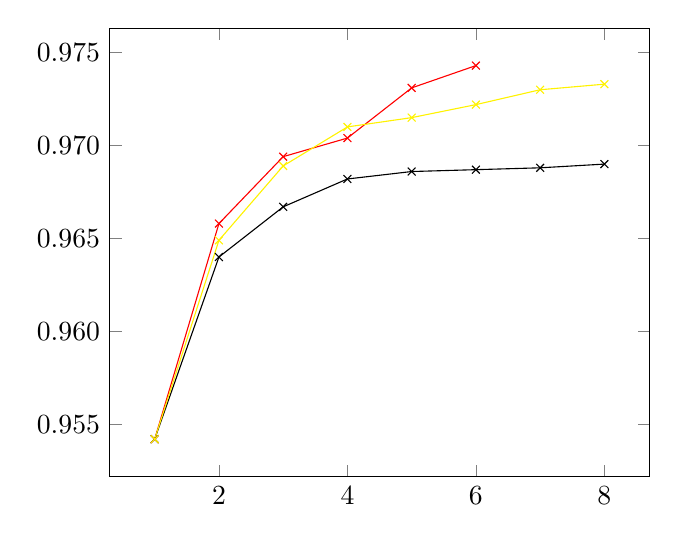
\begin{tikzpicture}
\begin{axis}[y tick label style={ /pgf/number format/.cd, fixed, fixed zerofill, precision=3 }]
    \addplot[color=red,mark=x] coordinates {
        (1.000000 ,  1- 0.045800)
        (2.000000 ,  1- 0.034200)
        (3.000000 ,  1- 0.030600)
        (4.000000 ,  1- 0.029600)
        (5.000000 ,  1- 0.026900)
        (6.000000 ,  1- 0.025700)
    };
    % 0.5 0.969
    \addplot[color=black,mark=x] coordinates {
        (1.000000  , 1-0.045800)
        (2.000000  , 1-0.036000)
        (3.000000  , 1-0.033300)
        (4.000000  , 1-0.031800)
        (5.000000  , 1-0.031400)
        (6.000000  , 1-0.031300)
        (7.000000  , 1-0.031200)
        (8.000000  , 1-0.031000)
    };
    % 0.75 0.973
    \addplot[color=yellow,mark=x] coordinates {
        (1.000000,   1-0.045800)
        (2.000000,   1-0.035100)
        (3.000000,   1-0.031100)
        (4.000000,   1-0.029000)
        (5.000000,   1-0.028500)
        (6.000000,   1-0.027800)
        (7.000000,   1-0.027000)
        (8.000000,   1-0.026700)
    };
\end{axis}
\end{tikzpicture}
\end{center}

Wyniki te sugerują zwiększenie początkowego współczynnika uczenia.
Przeprowadziłem ekperymenty dla zwiększonego tego współczynnika ze spadkiem 0.75
raza z każdą epoką.
Wyniki eksperymentów (pomarańczowy - pocz. wsp. uczenia równy 0.01, zielony - 0.02):

\begin{center}
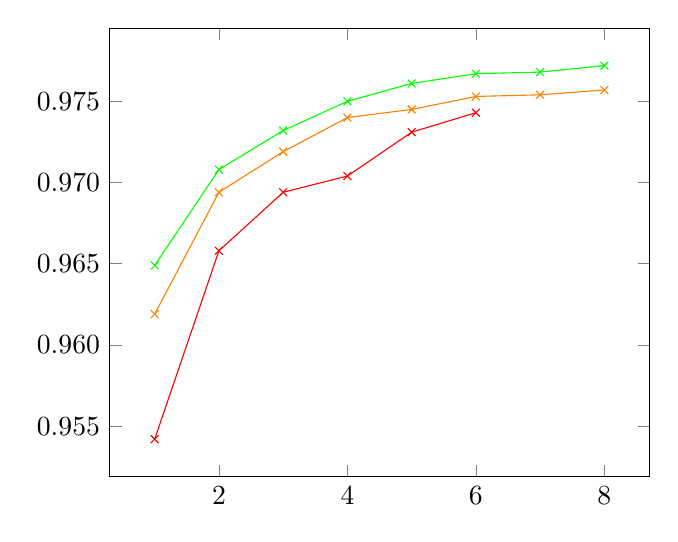
\begin{tikzpicture}
\begin{axis}[y tick label style={ /pgf/number format/.cd, fixed, fixed zerofill, precision=3 }]
    \addplot[color=red,mark=x] coordinates {
        (1.000000 ,  1- 0.045800)
        (2.000000 ,  1- 0.034200)
        (3.000000 ,  1- 0.030600)
        (4.000000 ,  1- 0.029600)
        (5.000000 ,  1- 0.026900)
        (6.000000 ,  1- 0.025700)
    };
    % 0.5 0.969
    \addplot[color=orange,mark=x] coordinates {
        (1.000000  ,1- 0.038100)
        (2.000000  ,1- 0.030600)
        (3.000000  ,1- 0.028100)
        (4.000000  ,1- 0.026000)
        (5.000000  ,1- 0.025500)
        (6.000000  ,1- 0.024700)
        (7.000000  ,1- 0.024600)
        (8.000000  ,1- 0.024300)

    };
    % 0.75 0.973
    \addplot[color=green,mark=x] coordinates {
        (1.000000  ,1- 0.035100)
        (2.000000  ,1- 0.029200)
        (3.000000  ,1- 0.026800)
        (4.000000  ,1- 0.025000)
        (5.000000  ,1- 0.023900)
        (6.000000  ,1- 0.023300)
        (7.000000  ,1- 0.023200)
        (8.000000  ,1- 0.022800)

    };
\end{axis}
\end{tikzpicture}
\end{center}

Ostatecznie dla pocz. wsp. uczenia 0.02 udało się uzyskać precyzję
0.977 na zbiorze testowym (i 0.986 na trenującym).
Macierz pomyłek na zbiorze testowym dla tej sieci pokazana w tabeli \ref{table:confusion1}.

% -----------------Test set results
% ans =
% 
%    1.000000   0.035100
%    2.000000   0.029200
%    3.000000   0.026800
%    4.000000   0.025000
%    5.000000   0.023900
%    6.000000   0.023300
%    7.000000   0.023200
%    8.000000   0.022800
% 
% ans =
% 
%       1      2      3      4      5      6      7      8      9     10     11
%     975      1      1      0      0      0      0      1      2      0      0
%       0   1126      3      1      0      0      1      0      4      0      0
%       4      2   1003      5      1      0      2      5      8      2      0
%       0      0      5    985      0      8      0      4      4      4      0
%       2      0      0      0    959      0      5      0      1     15      0
%       3      1      1      8      1    868      5      2      3      0      0
%       7      3      0      1      2      6    933      0      6      0      0
%       2      2     14      2      2      1      0    997      2      6      0
%       4      0      1      2      3      2      1      3    954      4      0
%       4      5      0      5      9      1      1      5      7    972      0
% 
% ans =
% 
%    0.97720   0.02280   0.00000
% 
% -----------------Training set results
% ans =
% 
%       1      2      3      4      5      6      7      8      9     10     11
%    5882      1      1      2      1      1      6      1     24      4      0
%       1   6679     23      4      9      1      2      7     14      2      0
%      18     14   5862      8      6      0      3     14     27      6      0
%       1      4     31   6004      0     13      1     16     40     21      0
%       5      9      3      0   5777      0     11      4      3     30      0
%      10      6      4     27      7   5322     20      1     15      9      0
%      12      8      1      0      5     13   5866      0     13      0      0
%       1     18     24      1     11      0      1   6172      4     33      0
%      10     19      6      8      4      3      6      2   5783     10      0
%      10      5      1     25     16     10      3     17     23   5839      0
% 
% ans =
% 
%    0.98643   0.01357   0.00000


\begin{table}[!hbt]
    \caption{Macierz pomyłek dla sieci z 200 neuronami w warstwie ukrytej
    Wiersze odpowiadają odpowiedziom klasyfikatora (a kolumny -- "ground truth").
    \label{table:confusion1}
    }
\footnotesize
\begin{center}
    \begin{tabular}{ 
        |@{\hskip3pt}c@{\hskip3pt}
        |@{\hskip3pt}c@{\hskip3pt}
        |@{\hskip3pt}c@{\hskip3pt}
        |@{\hskip3pt}c@{\hskip3pt}
        |@{\hskip3pt}c@{\hskip3pt}
        |@{\hskip3pt}c@{\hskip3pt}
        |@{\hskip3pt}c@{\hskip3pt}
        |@{\hskip3pt}c@{\hskip3pt}
        |@{\hskip3pt}c@{\hskip3pt}
        |@{\hskip3pt}c@{\hskip3pt}
        |@{\hskip3pt}c@{\hskip3pt}|
        }
    \hline
- &         0&     1&     2&     3&     4&     5&     6&     7&     8&    9 \\
    \hline
0 &       975&     1&     1&     0&     0&     0&     0&     1&     2&     0 \\
1 &         0&  1126&     3&     1&     0&     0&     1&     0&     4&     0 \\
2 &         4&     2&  1003&     5&     1&     0&     2&     5&     8&     2 \\
3 &         0&     0&     5&   985&     0&     8&     0&     4&     4&     4 \\
4 &         2&     0&     0&     0&   959&     0&     5&     0&     1&    15 \\
5 &         3&     1&     1&     8&     1&   868&     5&     2&     3&     0 \\
6 &         7&     3&     0&     1&     2&     6&   933&     0&     6&     0 \\
7 &         2&     2&    14&     2&     2&     1&     0&   997&     2&     6 \\
8 &         4&     0&     1&     2&     3&     2&     1&     3&   954&     4 \\
9&         4&     5&     0&     5&     9&     1&     1&     5&     7&   972 \\

    \hline
    \end{tabular}
\end{center}
\end{table}

\section{Zmiana liczności neuronów w warstwie ukrytej}

Używając współczynnika uczenia 0.02 i opadania 0.75 na epokę,
przeprowadziłem 2 eksperymenty z innymi ilościami neuronów w warstwie ukrytej.
Wyniki eksperymentów (
niebieski -- 400 neuronów,
zielony -- 200 (z poprzedzniego eksperymentu),
szary -- 100,
i czerwony -- model podstawowy):

\begin{center}
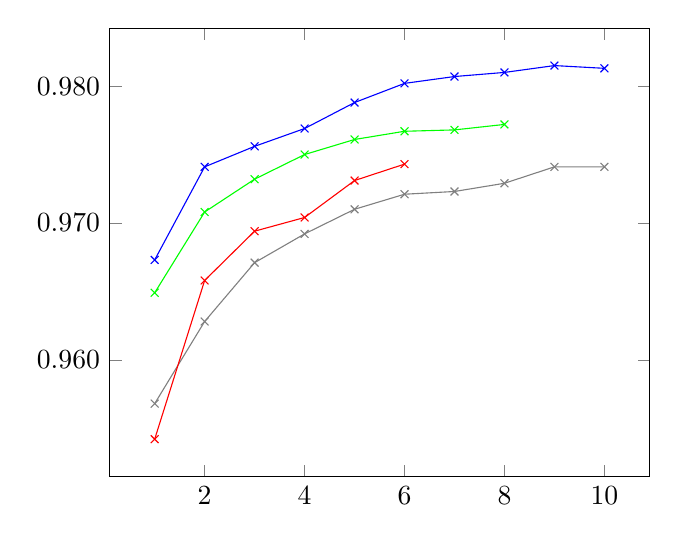
\begin{tikzpicture}
\begin{axis}[y tick label style={ /pgf/number format/.cd, fixed, fixed zerofill, precision=3 }]
    % 400
    \addplot[color=blue,mark=x] coordinates {
        (     1.000000   , 1- 0.032700)
        (     2.000000   , 1- 0.025900)
        (     3.000000   , 1- 0.024400)
        (     4.000000   , 1- 0.023100)
        (     5.000000   , 1- 0.021200)
        (     6.000000   , 1- 0.019800)
        (     7.000000   , 1- 0.019300)
        (     8.000000   , 1- 0.019000)
        (     9.000000   , 1- 0.018500)
        (    10.000000   , 1- 0.018700)
    };
    % 100
    \addplot[color=gray,mark=x] coordinates {
        (    1.000000 , 1- 0.043200)
        (    2.000000 , 1- 0.037200)
        (    3.000000 , 1- 0.032900)
        (    4.000000 , 1- 0.030800)
        (    5.000000 , 1- 0.029000)
        (    6.000000 , 1- 0.027900)
        (    7.000000 , 1- 0.027700)
        (    8.000000 , 1- 0.027100)
        (    9.000000 , 1- 0.025900)
        (   10.000000 , 1- 0.025900)
    };

    % 0.75 0.973
    \addplot[color=green,mark=x] coordinates {
        (1.000000  ,1- 0.035100)
        (2.000000  ,1- 0.029200)
        (3.000000  ,1- 0.026800)
        (4.000000  ,1- 0.025000)
        (5.000000  ,1- 0.023900)
        (6.000000  ,1- 0.023300)
        (7.000000  ,1- 0.023200)
        (8.000000  ,1- 0.022800)

    };

    \addplot[color=red,mark=x] coordinates {
        (1.000000 ,  1- 0.045800)
        (2.000000 ,  1- 0.034200)
        (3.000000 ,  1- 0.030600)
        (4.000000 ,  1- 0.029600)
        (5.000000 ,  1- 0.026900)
        (6.000000 ,  1- 0.025700)
    };
\end{axis}
\end{tikzpicture}
\end{center}

Sieć z 400 neuronami ukrytymi osiąga precyzję 0.981 na zbiorze testowym i 0.991 na trenującym.
Jak widać, pod koniec uczenia precyzja lekko spada -- najprawdopodobniej zaczyna się overfitting.
Macierz pomyłek na zbiorze testowym jest w tabeli \ref{table:confusion2},
a na trenującym w tabeli \ref{table:confusion3}.



\begin{table}[!hbt]
    \caption{Macierz pomyłek na zbiorze testowym dla sieci z 400 neuronami w warstwie ukrytej
    Wiersze odpowiadają odpowiedziom klasyfikatora (a kolumny -- "ground truth").
    \label{table:confusion2}
    }
\footnotesize
\begin{center}
    \begin{tabular}{ 
        |@{\hskip3pt}c@{\hskip3pt}
        |@{\hskip3pt}c@{\hskip3pt}
        |@{\hskip3pt}c@{\hskip3pt}
        |@{\hskip3pt}c@{\hskip3pt}
        |@{\hskip3pt}c@{\hskip3pt}
        |@{\hskip3pt}c@{\hskip3pt}
        |@{\hskip3pt}c@{\hskip3pt}
        |@{\hskip3pt}c@{\hskip3pt}
        |@{\hskip3pt}c@{\hskip3pt}
        |@{\hskip3pt}c@{\hskip3pt}
        |@{\hskip3pt}c@{\hskip3pt}|
        }
    \hline
- &         0&     1&     2&     3&     4&     5&     6&     7&     8&    9 \\
    \hline
0   & 972&     0 &    0&     0&     0&     1&     4&     1&     2&     0 \\
1   &   1&  1127 &    2&     2&     0&     1&     1&     0&     1&     0 \\
2   &   4&     2 & 1012&     3&     1&     0&     1&     5&     4&     0 \\
3   &   0&     0 &    5&   991&     0&     4&     0&     4&     4&     2 \\
4   &   2&     0 &    2&     0&   959&     0&     3&     0&     1&    15 \\
5   &   3&     0 &    0&     8&     0&   868&     6&     2&     4&     1 \\
6   &   5&     3 &    0&     1&     2&     3&   939&     0&     5&     0 \\
7   &   1&     4 &    7&     0&     2&     0&     0&  1007&     2&     5 \\
8   &   3&     0 &    1&     2&     2&     2&     2&     2&   958&     2 \\
9  &   4&     3 &    0&     3&     7&     2&     1&     4&     5&   980 \\
    \hline
    \end{tabular}
\end{center}
\end{table}

\begin{table}[!hbt]
    \caption{Macierz pomyłek na zbiorze trenującym dla sieci z 400 neuronami w warstwie ukrytej
    Wiersze odpowiadają odpowiedziom klasyfikatora (a kolumny -- "ground truth").
    \label{table:confusion3}
    }
\footnotesize
\begin{center}
    \begin{tabular}{ 
        |@{\hskip3pt}c@{\hskip3pt}
        |@{\hskip3pt}c@{\hskip3pt}
        |@{\hskip3pt}c@{\hskip3pt}
        |@{\hskip3pt}c@{\hskip3pt}
        |@{\hskip3pt}c@{\hskip3pt}
        |@{\hskip3pt}c@{\hskip3pt}
        |@{\hskip3pt}c@{\hskip3pt}
        |@{\hskip3pt}c@{\hskip3pt}
        |@{\hskip3pt}c@{\hskip3pt}
        |@{\hskip3pt}c@{\hskip3pt}
        |@{\hskip3pt}c@{\hskip3pt}|
        }
    \hline
- &         0&     1&     2&     3&     4&     5&     6&     7&     8&    9 \\
    \hline
0   &5902&     1&     0&     0&     1&     1&     5&     0&    11&     2 \\
1   &   2&  6700&    14&     2&     4&     1&     1&     7&     8&     3 \\
2   &   8&     4&  5916&     5&     2&     0&     1&     9&    11&     2 \\
3   &   2&     0&    14&  6058&     0&     7&     1&    14&    20&    15 \\
4   &   4&     7&     3&     0&  5794&     0&     8&     2&     0&    24 \\
5   &   4&     3&     2&     8&     1&  5376&    13&     1&     7&     6 \\
6   &  10&     5&     0&     0&     2&     9&  5886&     0&     6&     0 \\
7   &   1&    13&    16&     0&     7&     0&     1&  6209&     4&    14 \\
8   &   9&    13&     2&     3&     3&     2&     6&     1&  5805&     7 \\
9  &   5&     4&     0&    10&    13&     8&     2&    17&    17&  5873 \\
    \hline
    \end{tabular}
\end{center}
\end{table}


\section{Końcowy komentarz}

W przeprowadzonych eksperymentach istotym problemem jest wydajność implementacji.
Uczenie sieci jest przeprowadzone bez użycia GPU, w dotatku na 1 wątku. 
Prawdopodobnie implementacja octave (nie ważne na czym skompilowana)
nie korzysta z pełni możliwości jednoski wektorowej procesora przy mnożeniu macierzy.
Z tych powodów uczenie bardzo małego prostego modelu,
dla bardzo małego i prostego zbioru jak MNIST jest bardzo wolne
(czas rzędu godziny na 1 model zamiast np. minuty)
i eksperymentowanie staje się bardziej uciążliwe.

Inną niedogodnością jest wpisywanie ręcznie wzorów na pohodne funkcji straty po wagach.
Współcześnie istnieje wiele narzędzi do automatycznego obliczania pochodnej
zadanej funkcji po zadanej zmiennej (np. wagach warstwy) --
model jest reprezentowany przez graf.

Bez naruszania założenia, że architektura ma 2 warstwy fully connected --
modyfikacje jakie nalerzało by dalej sprawdzić (bo zreguły się sprawdzają),
to przepuszczenie wyjścia sieci przez softmax, użycie entropii wzajemnej jako funkcji straty,
oraz zastosowanie batch normalization (w tym oczywiście uczenie w mini-batchach) lub dropout.

\end{document}


% 100
% -----------------Test set results
% ans =
% 
%     1.000000    0.043200
%     2.000000    0.037200
%     3.000000    0.032900
%     4.000000    0.030800
%     5.000000    0.029000
%     6.000000    0.027900
%     7.000000    0.027700
%     8.000000    0.027100
%     9.000000    0.025900
%    10.000000    0.025900
% 
% ans =
% 
%       1      2      3      4      5      6      7      8      9     10     11
%     972      0      0      0      0      0      1      2      4      1      0
%       1   1124      2      2      0      2      2      0      2      0      0
%       4      3    999      3      2      0      1      8      9      3      0
%       0      0      8    983      0      3      0      4      7      5      0
%       1      0      4      0    954      0      4      0      1     18      0
%       3      0      0      6      1    864      7      3      6      2      0
%       7      3      0      0      5      4    933      0      6      0      0
%       1      2     14      1      4      0      0    993      3     10      0
%       4      1      1      0      3      4      2      2    952      5      0
%       3      7      0      7      8      2      1      5      9    967      0
% 
% ans =
% 
%    0.97410   0.02590   0.00000
% 
% -----------------Training set results
% ans =
% 
%       1      2      3      4      5      6      7      8      9     10     11
%    5862      1      1      2      4      1     10      1     37      4      0
%       3   6681     20      2      7      0      1      9     16      3      0
%      12      5   5868     10      5      0      7     19     28      4      0
%       5      5     36   5954      2     24      1     30     51     23      0
%       7      9      3      0   5724      0     17      7      7     68      0
%      12      4      7     26      8   5318     18      2     15     11      0
%      14      7      1      0      5     20   5849      0     21      1      0
%       1     24     21      0     14      1      2   6144      6     52      0
%       9     23     10      7      7      9     14      1   5744     27      0
%      12      4      1     27     29      9      2     23     29   5813      0
% 
% ans =
% 
%    0.98262   0.01738   0.00000


% BLUE
% -----------------Test set results
% ans =
% 
%     1.000000    0.032700
%     2.000000    0.025900
%     3.000000    0.024400
%     4.000000    0.023100
%     5.000000    0.021200
%     6.000000    0.019800
%     7.000000    0.019300
%     8.000000    0.019000
%     9.000000    0.018500
%    10.000000    0.018700
% 
% ans =
% 
%       1      2      3      4      5      6      7      8      9     10     11
%     972      0      0      0      0      1      4      1      2      0      0
%       1   1127      2      2      0      1      1      0      1      0      0
%       4      2   1012      3      1      0      1      5      4      0      0
%       0      0      5    991      0      4      0      4      4      2      0
%       2      0      2      0    959      0      3      0      1     15      0
%       3      0      0      8      0    868      6      2      4      1      0
%       5      3      0      1      2      3    939      0      5      0      0
%       1      4      7      0      2      0      0   1007      2      5      0
%       3      0      1      2      2      2      2      2    958      2      0
%       4      3      0      3      7      2      1      4      5    980      0
% 
% ans =
% 
%    0.98130   0.01870   0.00000
% 
% -----------------Training set results
% ans =
% 
%       1      2      3      4      5      6      7      8      9     10     11
%    5902      1      0      0      1      1      5      0     11      2      0
%       2   6700     14      2      4      1      1      7      8      3      0
%       8      4   5916      5      2      0      1      9     11      2      0
%       2      0     14   6058      0      7      1     14     20     15      0
%       4      7      3      0   5794      0      8      2      0     24      0
%       4      3      2      8      1   5376     13      1      7      6      0
%      10      5      0      0      2      9   5886      0      6      0      0
%       1     13     16      0      7      0      1   6209      4     14      0
%       9     13      2      3      3      2      6      1   5805      7      0
%       5      4      0     10     13      8      2     17     17   5873      0
% 
% ans =
% 
%    0.99198   0.00802   0.00000
